%==============================================================================
% tento soubor pouzijte jako zaklad
% this file should be used as a base for the thesis
% Autoři / Authors: 2008 Michal Bidlo, 2019 Jaroslav Dytrych
% Kontakt pro dotazy a připomínky: sablona@fit.vutbr.cz
% Contact for questions and comments: sablona@fit.vutbr.cz
%==============================================================================
% kodovani: UTF-8 (zmena prikazem iconv, recode nebo cstocs)
% encoding: UTF-8 (you can change it by command iconv, recode or cstocs)
%------------------------------------------------------------------------------
% zpracování / processing: make, make pdf, make clean
%==============================================================================
% Soubory, které je nutné upravit nebo smazat: / Files which have to be edited or deleted:
%   projekt-20-literatura-bibliography.bib - literatura / bibliography
%   projekt-01-kapitoly-chapters.tex - obsah práce / the thesis content
%   projekt-01-kapitoly-chapters-en.tex - obsah práce v angličtině / the thesis content in English
%   projekt-30-prilohy-appendices.tex - přílohy / appendices
%   projekt-30-prilohy-appendices-en.tex - přílohy v angličtině / appendices in English
%==============================================================================
\documentclass[english]{fitthesis} % bez zadání - pro začátek práce, aby nebyl problém s překladem
%\documentclass[english]{fitthesis} % without assignment - for the work start to avoid compilation problem
%\documentclass[zadani]{fitthesis} % odevzdani do wisu a/nebo tisk s barevnými odkazy - odkazy jsou barevné
%\documentclass[english,zadani]{fitthesis} % for submission to the IS FIT and/or print with color links - links are color
%\documentclass[zadani,print]{fitthesis} % pro černobílý tisk - odkazy jsou černé
%\documentclass[english,zadani,print]{fitthesis} % for the black and white print - links are black
%\documentclass[zadani,cprint]{fitthesis} % pro barevný tisk - odkazy jsou černé, znak VUT barevný
%\documentclass[english,zadani,cprint]{fitthesis} % for the print - links are black, logo is color
% * Je-li práce psaná v anglickém jazyce, je zapotřebí u třídy použít 
%   parametr english následovně:
%   If thesis is written in English, it is necessary to use 
%   parameter english as follows:
%      \documentclass[english]{fitthesis}
% * Je-li práce psaná ve slovenském jazyce, je zapotřebí u třídy použít 
%   parametr slovak následovně:
%   If the work is written in the Slovak language, it is necessary 
%   to use parameter slovak as follows:
%      \documentclass[slovak]{fitthesis}
% * Je-li práce psaná v anglickém jazyce se slovenským abstraktem apod., 
%   je zapotřebí u třídy použít parametry english a enslovak následovně:
%   If the work is written in English with the Slovak abstract, etc., 
%   it is necessary to use parameters english and enslovak as follows:
%      \documentclass[english,enslovak]{fitthesis}

% Základní balíčky jsou dole v souboru šablony fitthesis.cls
% Basic packages are at the bottom of template file fitthesis.cls
% zde můžeme vložit vlastní balíčky / you can place own packages here

% Kompilace po částech (rychlejší, ale v náhledu nemusí být vše aktuální)
% Compilation piecewise (faster, but not all parts in preview will be up-to-date)
% \usepackage{subfiles}

% Nastavení cesty k obrázkům
% Setting of a path to the pictures
%\graphicspath{{obrazky-figures/}{./obrazky-figures/}}
%\graphicspath{{obrazky-figures/}{../obrazky-figures/}}

%---rm---------------
\renewcommand{\rmdefault}{lmr}%zavede Latin Modern Roman jako rm / set Latin Modern Roman as rm
%---sf---------------
\renewcommand{\sfdefault}{qhv}%zavede TeX Gyre Heros jako sf
%---tt------------
\renewcommand{\ttdefault}{lmtt}% zavede Latin Modern tt jako tt

% vypne funkci šablony, která automaticky nahrazuje uvozovky,
% aby nebyly prováděny nevhodné náhrady v popisech API apod.
% disables function of the template which replaces quotation marks
% to avoid unnecessary replacements in the API descriptions etc.
\csdoublequotesoff



\usepackage{amsmath}
\usepackage{caption}
\usepackage{makecell}
\usepackage{multirow}
\usepackage{subcaption}
\usepackage{url}


% =======================================================================
% balíček "hyperref" vytváří klikací odkazy v pdf, pokud tedy použijeme pdflatex
% problém je, že balíček hyperref musí být uveden jako poslední, takže nemůže
% být v šabloně
% "hyperref" package create clickable links in pdf if you are using pdflatex.
% Problem is that this package have to be introduced as the last one so it 
% can not be placed in the template file.
\ifWis
\ifx\pdfoutput\undefined % nejedeme pod pdflatexem / we are not using pdflatex
\else
  \usepackage{color}
  \usepackage[unicode,colorlinks,hyperindex,plainpages=false,pdftex]{hyperref}
  \definecolor{hrcolor-ref}{RGB}{223,52,30}
  \definecolor{hrcolor-cite}{HTML}{2F8F00}
  \definecolor{hrcolor-urls}{HTML}{092EAB}
  \hypersetup{
	linkcolor=hrcolor-ref,
	citecolor=hrcolor-cite,
	filecolor=magenta,
	urlcolor=hrcolor-urls
  }
  \def\pdfBorderAttrs{/Border [0 0 0] }  % bez okrajů kolem odkazů / without margins around links
  \pdfcompresslevel=9
\fi
\else % pro tisk budou odkazy, na které se dá klikat, černé / for the print clickable links will be black
\ifx\pdfoutput\undefined % nejedeme pod pdflatexem / we are not using pdflatex
\else
  \usepackage{color}
  \usepackage[unicode,colorlinks,hyperindex,plainpages=false,pdftex,urlcolor=black,linkcolor=black,citecolor=black]{hyperref}
  \definecolor{links}{rgb}{0,0,0}
  \definecolor{anchors}{rgb}{0,0,0}
  \def\AnchorColor{anchors}
  \def\LinkColor{links}
  \def\pdfBorderAttrs{/Border [0 0 0] } % bez okrajů kolem odkazů / without margins around links
  \pdfcompresslevel=9
\fi
\fi
% Řešení problému, kdy klikací odkazy na obrázky vedou za obrázek
% This solves the problems with links which leads after the picture
\usepackage[all]{hypcap}

% Informace o práci/projektu / Information about the thesis
%---------------------------------------------------------------------------
\projectinfo{
  %Prace / Thesis
  project={SP},            %typ práce BP/SP/DP/DR  / thesis type (SP = term project)
  year={2021},             % rok odevzdání / year of submission
  date=\today,             % datum odevzdání / submission date
  %Nazev prace / thesis title
  title.cs={Detekcia anomálií ICS komunikacie pomocou štatistických modelov},  % název práce v češtině či slovenštině (dle zadání) / thesis title in czech language (according to assignment)
  title.en={Anomaly detection of ICS traffic using statistical features}, % název práce v angličtině / thesis title in english
  %title.length={14.5cm}, % nastavení délky bloku s titulkem pro úpravu zalomení řádku (lze definovat zde nebo níže) / setting the length of a block with a thesis title for adjusting a line break (can be defined here or below)
  %sectitle.length={14.5cm}, % nastavení délky bloku s druhým titulkem pro úpravu zalomení řádku (lze definovat zde nebo níže) / setting the length of a block with a second thesis title for adjusting a line break (can be defined here or below)
  %dectitle.length={14.5cm}, % nastavení délky bloku s titulkem nad prohlášením pro úpravu zalomení řádku (lze definovat zde nebo níže) / setting the length of a block with a thesis title above declaration for adjusting a line break (can be defined here or below)
  %Autor / Author
  author.name={Patrik},   % jméno autora / author name
  author.surname={Németh},   % příjmení autora / author surname 
  %author.title.p={Bc.}, % titul před jménem (nepovinné) / title before the name (optional)
  %author.title.a={Ph.D.}, % titul za jménem (nepovinné) / title after the name (optional)
  %Ustav / Department
  department={UIFS}, % doplňte příslušnou zkratku dle ústavu na zadání: UPSY/UIFS/UITS/UPGM / fill in appropriate abbreviation of the department according to assignment: UPSY/UIFS/UITS/UPGM
  % Školitel / supervisor
  supervisor.name={Jméno},   % jméno školitele / supervisor name 
  supervisor.surname={Příjmení},   % příjmení školitele / supervisor surname
  supervisor.title.p={prof. RNDr.},   %titul před jménem (nepovinné) / title before the name (optional)
  supervisor.title.a={Ph.D.},    %titul za jménem (nepovinné) / title after the name (optional)
  % Klíčová slova / keywords
  keywords.cs={Sem budou zapsána jednotlivá klíčová slova v českém (slovenském) jazyce, oddělená čárkami.}, % klíčová slova v českém či slovenském jazyce / keywords in czech or slovak language
  keywords.en={Sem budou zapsána jednotlivá klíčová slova v anglickém jazyce, oddělená čárkami.}, % klíčová slova v anglickém jazyce / keywords in english
  %keywords.en={Here, individual keywords separated by commas will be written in English.},
  % Abstrakt / Abstract
  abstract.cs={Do tohoto odstavce bude zapsán výtah (abstrakt) práce v českém (slovenském) jazyce.}, % abstrakt v českém či slovenském jazyce / abstract in czech or slovak language
  abstract.en={Do tohoto odstavce bude zapsán výtah (abstrakt) práce v anglickém jazyce.}, % abstrakt v anglickém jazyce / abstract in english
  %abstract.en={An abstract of the work in English will be written in this paragraph.},
  % Prohlášení (u anglicky psané práce anglicky, u slovensky psané práce slovensky) / Declaration (for thesis in english should be in english)
  declaration={Prohlašuji, že jsem tuto bakalářskou práci vypracoval samostatně pod vedením pana X...
Další informace mi poskytli...
Uvedl jsem všechny literární prameny, publikace a další zdroje, ze kterých jsem čerpal.},
  %declaration={I hereby declare that this Bachelor's thesis was prepared as an original work by the author under the supervision of Mr. X
% The supplementary information was provided by Mr. Y
% I have listed all the literary sources, publications and other sources, which were used during the preparation of this thesis.},
  % Poděkování (nepovinné, nejlépe v jazyce práce) / Acknowledgement (optional, ideally in the language of the thesis)
  acknowledgment={V této sekci je možno uvést poděkování vedoucímu práce a těm, kteří poskytli odbornou pomoc
(externí zadavatel, konzultant apod.).},
  %acknowledgment={Here it is possible to express thanks to the supervisor and to the people which provided professional help
%(external submitter, consultant, etc.).},
  % Rozšířený abstrakt (cca 3 normostrany) - lze definovat zde nebo níže / Extended abstract (approximately 3 standard pages) - can be defined here or below
  %extendedabstract={Do tohoto odstavce bude zapsán rozšířený výtah (abstrakt) práce v českém (slovenském) jazyce.},
  %extabstract.odd={true}, % Začít rozšířený abstrakt na liché stránce? / Should extended abstract start on the odd page?
  %faculty={FIT}, % FIT/FEKT/FSI/FA/FCH/FP/FAST/FAVU/USI/DEF
  faculty.cs={Fakulta informačních technologií}, % Fakulta v češtině - pro využití této položky výše zvolte fakultu DEF / Faculty in Czech - for use of this entry select DEF above
  faculty.en={Faculty of Information Technology}, % Fakulta v angličtině - pro využití této položky výše zvolte fakultu DEF / Faculty in English - for use of this entry select DEF above
  department.cs={Ústav matematiky}, % Ústav v češtině - pro využití této položky výše zvolte ústav DEF nebo jej zakomentujte / Department in Czech - for use of this entry select DEF above or comment it out
  department.en={Institute of Mathematics} % Ústav v angličtině - pro využití této položky výše zvolte ústav DEF nebo jej zakomentujte / Department in English - for use of this entry select DEF above or comment it out
}

% Rozšířený abstrakt (cca 3 normostrany) - lze definovat zde nebo výše / Extended abstract (approximately 3 standard pages) - can be defined here or above
%\extendedabstract{Do tohoto odstavce bude zapsán výtah (abstrakt) práce v českém (slovenském) jazyce.}
% Začít rozšířený abstrakt na liché stránce? / Should extended abstract start on the odd page?
%\extabstractodd{true}

% nastavení délky bloku s titulkem pro úpravu zalomení řádku - lze definovat zde nebo výše / setting the length of a block with a thesis title for adjusting a line break - can be defined here or above
%\titlelength{14.5cm}
% nastavení délky bloku s druhým titulkem pro úpravu zalomení řádku - lze definovat zde nebo výše / setting the length of a block with a second thesis title for adjusting a line break - can be defined here or above
%\sectitlelength{14.5cm}
% nastavení délky bloku s titulkem nad prohlášením pro úpravu zalomení řádku - lze definovat zde nebo výše / setting the length of a block with a thesis title above declaration for adjusting a line break - can be defined here or above
%\dectitlelength{14.5cm}

% řeší první/poslední řádek odstavce na předchozí/následující stránce
% solves first/last row of the paragraph on the previous/next page
\clubpenalty=10000
\widowpenalty=10000

% checklist
\newlist{checklist}{itemize}{1}
\setlist[checklist]{label=$\square$}

% Nechcete-li, aby se u oboustranného tisku roztahovaly mezery pro zaplnění stránky, odkomentujte následující řádek / If you do not want enlarged spacing for filling of the pages in case of duplex printing, uncomment the following line
% \raggedbottom

\begin{document}
  % Vysazeni titulnich stran / Typesetting of the title pages
  % ----------------------------------------------
  \maketitle
  % Obsah
  % ----------------------------------------------
  \setlength{\parskip}{0pt}

  {\hypersetup{hidelinks}\tableofcontents}
  
  % Seznam obrazku a tabulek (pokud prace obsahuje velke mnozstvi obrazku, tak se to hodi)
  % List of figures and list of tables (if the thesis contains a lot of pictures, it is good)
  \ifczech
    \renewcommand\listfigurename{Seznam obrázků}
  \fi
  \ifslovak
    \renewcommand\listfigurename{Zoznam obrázkov}
  \fi
  % {\hypersetup{hidelinks}\listoffigures}
  
  \ifczech
    \renewcommand\listtablename{Seznam tabulek}
  \fi
  \ifslovak
    \renewcommand\listtablename{Zoznam tabuliek}
  \fi
  % {\hypersetup{hidelinks}\listoftables}

  \ifODSAZ
    \setlength{\parskip}{0.5\bigskipamount}
  \else
    \setlength{\parskip}{0pt}
  \fi

  % vynechani stranky v oboustrannem rezimu
  % Skip the page in the two-sided mode
  \iftwoside
    \cleardoublepage
  \fi

  % Text prace / Thesis text
  % ----------------------------------------------
  \ifenglish
    \newcommand{\code}{\texttt}
\renewcommand\theadalign{bc}
\renewcommand\theadfont{\bfseries}
\renewcommand\theadgape{\Gape[4pt]}
\renewcommand\cellgape{\Gape[4pt]}

\chapter{The project}
\section{Anomaly detection in network traffic}
System administrators often need to quickly identify causes behind anomalous network traffic. This however can be very difficult to do manually,
and for this reason network analysis tools are used in order to easier identify causes behind anomalous behaviour. This project attempts to replicate
a recently published method of network anomaly detection for \emph{ICS} (Industrial Control System) traffic \cite{burgetova_anomaly}.

ICS communication is generally well protected against external threats of cyberattacks, however as soon as an endpoint is compromised,
the attack prevention mechanisms begin to fail \cite{burgetova_anomaly}. ICS traffic is generally highly stable in packet exchange frequency and
intermediate node count, and therefore can be subject to statistical modeling based on these features.
As an attacker may initiate various attacks from the compromised node, particularly by tampering with packet counts, a model of normal traffic communication
may be used to discriminate the anomalous traffic.


\section{Standard IEC 60870-5-104}
The IEC 60870 set of standards define systems used for telecontrol in electrical engineering and power system automation applications,
part 5 of which provides a communication profile for sending basic telecontrol messages between a central telecontrol station and telecontrol outstations.
This communication profile uses permanent and directly connected data circuits \cite{IEC104}. Part 5 of these standards consists of multiple
additional parts and this project focuses on parts 101 and its extension, 104 (further as IEC 104).

\subsection{Packet structure}
The IEC 104 packets are encapsulated within TCP/IP packets providing reliable delivery. Every IEC 104 packet
contains an \emph{APDU} (Application Protocol Data Unit), which encapsulates two other sections.
An \emph{APCI} (Application Protocol Control Information) section of a fixed length of 6 bytes and a variable length \emph{ASDU} section.

Each APCI starts with a 0x68 byte followed by an 8-bit value of the length of the APDU (this length does not include the first two bytes of the APCI).
The final four bytes of the APCI are 8-bit control fields. The two least significant bits of the first control field signify the type of the telecontrol message.
The type may be one of three formats - I, S or U and only the I format contains an ASDU. An APDU always contains an APCI.
The ASDU is a variable length data structure, consisting of two sections. A \emph{DUI} (Data Unit Identifier) section with a fixed length of 6 bytes and
a variable length data section \cite{mai2019iec}\cite{IEC104}. An illustraction of the packet structure can be seen in figure \ref{fig:packet_structure}.

\begin{figure}
  \centering
  \begin{subfigure}[b]{0.3\textwidth}
    \centering
    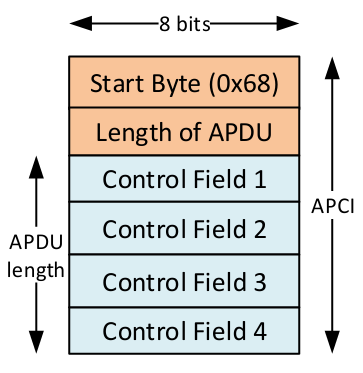
\includegraphics[width=\textwidth]{obrazky-figures/apdu_fixed_length.png}
    \caption{fixed length APDU}
    \label{fig:fixed_length_APDU}
  \end{subfigure}
  \hfill
  \begin{subfigure}[b]{0.3\textwidth}
    \centering
    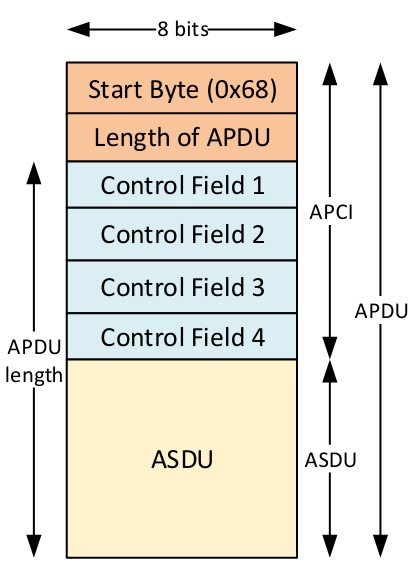
\includegraphics[width=\textwidth]{obrazky-figures/apdu_variable_length.png}
    \caption{variable length APDU}
    \label{fig:variable_length_APDU}
  \end{subfigure}
  \hfill
  \begin{subfigure}[b]{0.3\textwidth}
    \centering
    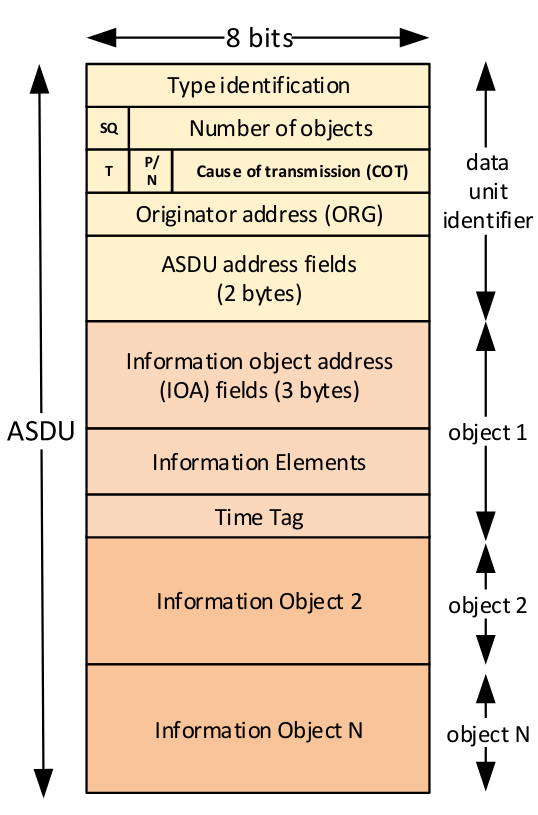
\includegraphics[width=\textwidth]{obrazky-figures/asdu.png}
    \caption{ASDU}
    \label{fig:ASDU}
  \end{subfigure}
  \caption{Visualization of the APCI and ASDU fields. Taken from \cite{IEC104}.}
  \label{fig:packet_structure}
\end{figure}

\section{The dataset and statistical modeling}
For this project the \code{mega104-17-12-18} dataset was used. The raw dataset contains over $150000$ packets captured over the course of
about $68$ hours. However, as we are only interested in IEC 104 communication, the irrelevant packets have been filtered out, which left us
with $58929$ IEC 104 packets in total. The dataset contains one master and one slave endpoint.

As described in \cite{burgetova_anomaly}, the inter arrival times of subsequent packets can be used for statistical modeling of
IEC 104 communication. These are acquired through the subtraction of arrival times of individual consecutive packets. The utilized pcap dataset contains metadata
with these packet arrival times, and therefore could be used for modeling. The direction of the packets can be classified by either the source and destination IP
addresses, or by the source and destination transport layer ports.
%// TODO dont know if this is correct: The specific classification of master-to-slave or slave-to-master directions is not
%important in the method put forward in \cite{burgetova_anomaly}, as the resulting statistical model does not differentiate between the two.

\subsection{Anomaly detection method}
The anomaly detection method used is the same as in \cite{burgetova_anomaly}. It utilizes the inter-arrival times of consecutive packets to build a
statistical model capable of detecting various anomalies in the network.
First the input dataset is split into two directions - communication from master to slave and from slave to master. This is done because the opposing
directions have different communication characteristics. The timing metadata is gathered and time differences for each direction are computed, such that
$\Delta t_{i} = \Delta t_{i+1} - \Delta t_{i}$. The result is a list of $\Delta t$ values of inter arrival times (this list will bereferred to as $\Delta T$).

\subsubsection{Split-points}
The used anomaly detection method hinges on the concept of a split-point. The split-point defines a suitable value in the range of
observed $\Delta t$ values. Its function is to split the $\Delta T$ list into two new lists - one, where $\Delta t < split\text{-}point$ and another,
where $\Delta t \geq split\text{-}point$. Before choosing a suitable split-point, four initial values per direction are computed - the $Q1$, $Q2$, $Q3$ quartiles
and the mean of $\Delta T$. The candidate split-points should be computed for any communication dataset individually, as the communication between various
devices has different characteristics, making it infeasable to use fixed split-point candidates. The $\Delta T$ list is to be split by each candidate
split-point as stated above.

\subsubsection{Time windows}
All of the gathered data based on the candidate split-points now needs to be grouped together into 5-minute windows based on the original packet
timestamps. The sizes of these windows are then computed (i.e. the number of packets per each 5 minute window). These window sizes are subsequently used to
choose the most suitable split-point for the dataset. The chosen split-point is the one that generated window sizes with the lowest standard deviation,
and which conforms to the condition $(mean(window\text{ }sizes) - 3*std(window\text{ }sizes)) > 0 $. The calculated standard deviation and mean belonging
to the chosen split-point is saved. Time window distributions for the from-master direction with split-point $8.0006$ and for the to-master direction
with split-point $11.1537$ are shown in figure \ref{fig:window_size_graphs}.

\subsubsection{The final profile}
The final profile is a 4-tuple of the following form:\\
$(split\text{-}point, \left\langle all^{-}, all^{+} \right\rangle,
\left\langle lt^{-}, lt^{+} \right\rangle, \left\langle geq^{-}, geq^{+} \right\rangle)$, where $split\text{-}point$ is the most suitable split-point,
and the three ranges denote the valid number of packets for any 5 minute window according to the three-sigma-rule, such that $all$ applies to the number of all packets
within a window, $lt$ applies to the number of packets with $\Delta t$ less than the split-point, and $geq$ applies to the the number of packets with $\Delta t$
greater or equal to the split-point. The three sigma rule defines the interval $\left\langle mean - 3\sigma , mean + 3\sigma \right\rangle$.

\begin{figure}
  \centering
  \begin{subfigure}[b]{0.49\textwidth}
    \centering
    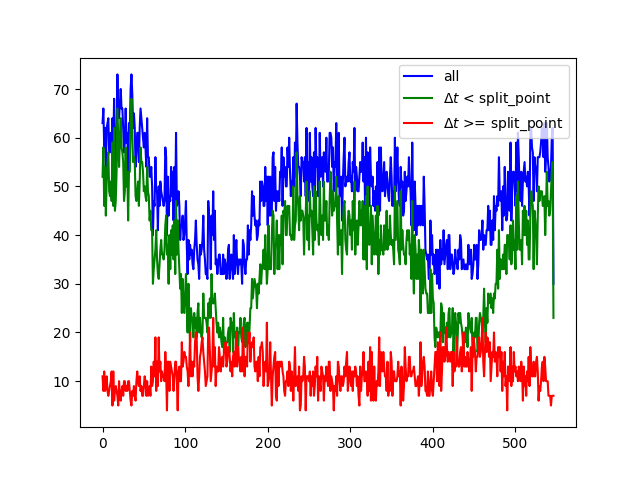
\includegraphics[width=\textwidth]{obrazky-figures/from_master.png}
    \caption{from master}
    \label{fig:master_slave}
  \end{subfigure}
  \hfill
  \begin{subfigure}[b]{0.49\textwidth}
    \centering
    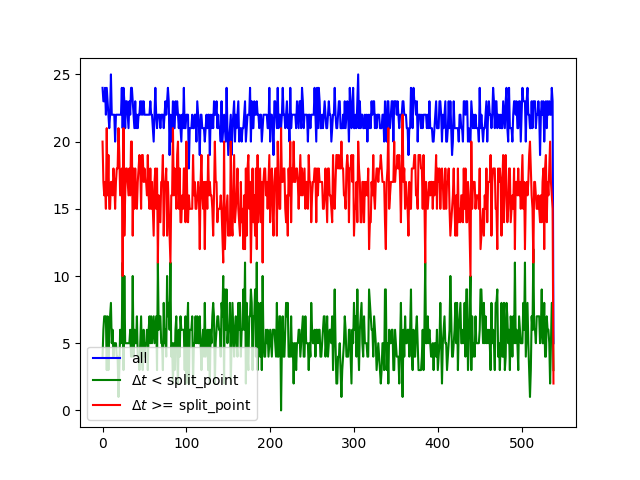
\includegraphics[width=\textwidth]{obrazky-figures/to_master.png}
    \caption{to master}
    \label{fig:slave_master}
  \end{subfigure}
  \caption{Window sizes in directions from and to master.}
  \label{fig:window_size_graphs}
\end{figure}

\section{Evaluation and conclusion}
The profile was built from two thirds of the provided dataset \code{mega104-17-12-18} and validated on the final third of the dataset. Table
\ref{tab:validation} shows the validation results for simple anomaly detection, where each time window outside the expected range is counted as
an anomaly.
In conclusion, we were able to partially reproduce the results of \cite{burgetova_anomaly}.

\begin{table}
  \centering
  \caption{Validation results for dataset \code{mega104-17-12-18}.}
  \begin{tabular}{| l | r | c | c |}
    \hline
    \thead{Direction} & \thead{Split\\category} & \thead{False\\Positives} & \thead{Accuracy} \\
    \hline
    \multirow{3}{1em}{from master} & $all$ & $1/277$ & $99.6390\%$ \\
      & $< split\text{-}point$ & $0/277$ & $100\%$ \\
      & $\geq split\text{-}point$ & $0/277$ & $100\%$ \\
    \hline
    \multirow{3}{1em}{to master} & $all$ & $1/269$ & $99.6283\%$ \\
      & $< split\text{-}point$ & $0/269$ & $100\%$ \\
      & $\geq split\text{-}point$ & $4/269$ & $98.5130\%$ \\
    \hline
  \end{tabular}
\end{table}\label{tab:validation}



  \else
    \input{projekt-01-kapitoly-chapters}
  \fi
  
  % Kompilace po částech (viz výše, nutno odkomentovat)
  % Compilation piecewise (see above, it is necessary to uncomment it)
  %\subfile{projekt-01-uvod-introduction}
  % ...
  %\subfile{chapters/projekt-05-conclusion}


  % Pouzita literatura / Bibliography
  % ----------------------------------------------
\ifslovak
  \makeatletter
  \def\@openbib@code{\addcontentsline{toc}{chapter}{Literatúra}}
  \makeatother
  \bibliographystyle{bib-styles/Pysny/skplain}
\else
  \ifczech
    \makeatletter
    \def\@openbib@code{\addcontentsline{toc}{chapter}{Literatura}}
    \makeatother
    \bibliographystyle{bib-styles/Pysny/czplain}
  \else 
    \makeatletter
    \def\@openbib@code{\addcontentsline{toc}{chapter}{Bibliography}}
    \makeatother
    \bibliographystyle{bib-styles/Pysny/enplain}
  %  \bibliographystyle{alpha}
  \fi
\fi
  \begin{flushleft}
  \bibliography{projekt-20-literatura-bibliography}
  \end{flushleft}

  % vynechani stranky v oboustrannem rezimu
  % Skip the page in the two-sided mode
  \iftwoside
    \cleardoublepage
  \fi

  % Prilohy / Appendices
  % ---------------------------------------------
  \appendix
\ifczech
  \renewcommand{\appendixpagename}{Přílohy}
  \renewcommand{\appendixtocname}{Přílohy}
  \renewcommand{\appendixname}{Příloha}
\fi
\ifslovak
  \renewcommand{\appendixpagename}{Prílohy}
  \renewcommand{\appendixtocname}{Prílohy}
  \renewcommand{\appendixname}{Príloha}
\fi
%  \appendixpage

% vynechani stranky v oboustrannem rezimu
% Skip the page in the two-sided mode
%\iftwoside
%  \cleardoublepage
%\fi
  
\ifslovak
%  \section*{Zoznam príloh}
%  \addcontentsline{toc}{section}{Zoznam príloh}
\else
  \ifczech
%    \section*{Seznam příloh}
%    \addcontentsline{toc}{section}{Seznam příloh}
  \else
%    \section*{List of Appendices}
%    \addcontentsline{toc}{section}{List of Appendices}
  \fi
\fi
  \startcontents[chapters]
  \setlength{\parskip}{0pt} 
  % seznam příloh / list of appendices
  % \printcontents[chapters]{l}{0}{\setcounter{tocdepth}{2}}
  
  \ifODSAZ
    \setlength{\parskip}{0.5\bigskipamount}
  \else
    \setlength{\parskip}{0pt}
  \fi
  
  % vynechani stranky v oboustrannem rezimu
  \iftwoside
    \cleardoublepage
  \fi
  
  % Přílohy / Appendices
  \ifenglish
    \input{projekt-30-prilohy-appendices-en}
  \else
    \input{projekt-30-prilohy-appendices}
  \fi
  
  % Kompilace po částech (viz výše, nutno odkomentovat)
  % Compilation piecewise (see above, it is necessary to uncomment it)
  %\subfile{projekt-30-prilohy-appendices}
  
\end{document}
